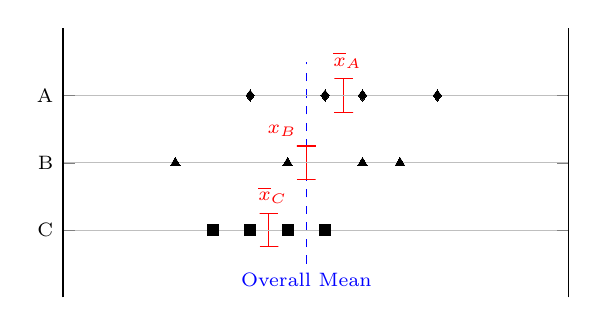
\begin{tikzpicture}
  \begin{axis}[
      axis x line*=bottom,
      xmin = 24, xmax = 37.5,
      ymin = 0, ymax = 4,
      xtick=\empty,
      ytick={1,2,3},
      yticklabels = {C,B,A},
      ticklabel style={font=\scriptsize},
      grid = major,
      axis on top,
%      hide y axis,
      hide x axis,
      height=5cm,
      width=8cm
    ]
    \addplot[mark=diamond*,line width=0mm] coordinates {  (32,3) (29,3) (34,3) (31,3) };
    \addplot[mark=triangle*,line width=0mm] coordinates { (30,2) (27,2) (33,2) (32,2) };
    \addplot[mark=square*,line width=0mm] coordinates { (28,1) (31,1) (29,1) (30,1) };
    \draw[blue,dashed] (axis cs: 30.5,0.5) node[below] {\scriptsize Overall Mean} -- (30.5,3.5);
    \draw[red] (axis cs: 31.25,2.75) -- (31.75,2.75) -- (31.5,2.75) -- (31.5,3.25) node[above] {\scriptsize $\,\,\overline{x}_A$} -- (31.25,3.25) -- (31.75,3.25);
    \draw[red] (axis cs: 30.25,1.75) -- (30.75,1.75) -- (30.5,1.75) -- (30.5,2.25) node[above left] {\scriptsize $\lverline{x}_B$} -- (30.25,2.25) -- (30.75,2.25);
    \draw[red] (axis cs: 29.25,0.75) -- (29.75,0.75) -- (29.5,0.75) -- (29.5,1.25) node[above] {\scriptsize $\,\,\overline{x}_C$} -- (29.25,1.25) -- (29.75,1.25);
    \draw[-stealth] (axis cs: -2.5,0.08) node[above left]  {\scriptsize $0.05$} to (axis cs: -2.25,0.06);
    \draw[line width=0.4mm,->] (axis cs: -3.626,0.03) node[above] {\scriptsize $t_{test}$} to (axis cs: -3.626,0);
  \end{axis}
\end{tikzpicture}